\documentclass{article}%
\usepackage[T1]{fontenc}%
\usepackage[utf8]{inputenc}%
\usepackage{lmodern}%
\usepackage{textcomp}%
\usepackage{lastpage}%
\usepackage[tmargin=1cm,lmargin=1cm]{geometry}%
\usepackage{graphicx}%
%
%
%
\begin{document}%
\normalsize%
\section{XcosDiagram}%
\label{sec:XcosDiagram}%
\begin{tabular}{|c|c|}%
\hline%
Name&Value\\%
\hline%
debugLevel&0\\%
\hline%
finalIntegrationTime&100000.0\\%
\hline%
integratorAbsoluteTolerance&1.0E{-}6\\%
\hline%
integratorRelativeTolerance&1.0E{-}6\\%
\hline%
toleranceOnTime&100001.0\\%
\hline%
maximumStepSize&0.0\\%
\hline%
realTimeScaling&0.0\\%
\hline%
solver&1.0\\%
\hline%
background&{-}1\\%
\hline%
gridEnabled&1\\%
\hline%
title&Untitled\\%
\hline%
\end{tabular}

%
\section{Basic info}%
\label{sec:Basic info}%
\begin{tabular}{|c|c|}%
\hline%
Name&Value\\%
\hline%
id&377a5292:16b0244b376:{-}7ff9\\%
\hline%
parent&0:2:0\\%
\hline%
interfaceFunctionName&ABS\_VALUE\\%
\hline%
blockType&c\\%
\hline%
dependsOnU&0\\%
\hline%
simulationFunctionName&absolute\_valueo\\%
\hline%
simulationFunctionType&C\_OR\_FORTRAN\\%
\hline%
style&ABS\_VALUE\\%
\hline%
\end{tabular}

%
\section{Absolute Value}%
\label{sec:Absolute Value}%


\begin{figure}[h!]%
\centering%
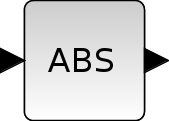
\includegraphics[width=120px]{/home/kyoya2212/fossee_2019/Rendering-simulation/images/ABS_VALUE.png}%
\caption{Absolute Value Block}%
\end{figure}

%
\end{document}